\chapter{Click Modular Router}
\thispagestyle{empty}

The \textbf{Click Modular Router} is a project that was born out of a paper by Eddie Kohler and other collaborators in 2000 \cite{Kohler2000}. It is still being given very sporadic, but important, updates by Kohler himself \href{https://github.com/kohler/click}{in his personal github repository}. It is designed to be a software architecture for building configurable routers. These routers are composed of simple packet routing modules, called \textit{elements}, that perform relatively straightforward functions. Click works by concatenating these elements (with possibly multiple inputs and outputs), in a meaningful way. This property makes it particularly easy to expand the software with user-defined elements, which was the case in this project.

Click configuration files, which specify the flow of packets by listing the elements and their respective connections, are written in their own, simple syntax. Element files in themselves use C++, with its own implementation of the C++ Standard Library, which contains equivalents to most of the STL data structures. 

The software is capable of running the router either at the user level or as a Linux kernel thread. Be advised that not all elements included in the software distribution can be executed at a kernel level. One of the original goals of this project was kernel integration of the resulting application, but unforeseen errors lead to debugging at a kernel level being out of the time scope devised for it. For further details, please refer to subsection \ref{k_int}.

Click has a significant learning curve, especially due to lack of documentation and online resources, so perseverance is advised.

\section{Why Click?}

The Click Modular Router software had already been identified as the option with most potential from before the start of the practice in itself by my supervisor, Mr. Bachhuber. However, part of the literature research needed included evaluating other options for the implementation of the application.

Alternatives seemed to be relatively scarce and deplorably out of date. The main ones identified were:
\begin{itemize}
\item X-kernel
\item Scout
\item OpenVZ
\end{itemize}

\href{http://www.cs.arizona.edu/projects/xkernel/}{\textit{X-kernel}} is a project that was mostly maintained by researchers from the University of Arizona. Its aim is to be an ''Object-based framework for implementing network protocols''. Most of its functionality was aimed at the TCP/IP protocol, and was deemed to lack the flexibility needed in order to process packets that did not expressly follow the protocol. I was also unable to find a reference or paper from this millennium, which further made it seem nonviable for the realization of the flusher.

\href{http://www.cs.arizona.edu/projects/scout/}{\textit{Scout}} was devised as a spin-off of X-kernel, also with support from University of Arizona personnel. It was described as being  a ''communication-oriented operating system targeted at network appliances''. Despite being operating system, which would probably grant some greater measure of speed or expediency, it was also seen as not fitting the specifications. This was in no small part due to the woeful lack of updates and the sorry state of its host website and documentation.

\href{https://openvz.org/}{\textit{OpenVZ}}, as discussed more thoroughly in a research paper by Doriguzzi et al \cite{DoriguzziCorin2011}, is a ''modified Linux kernel tree supporting virtualization, isolation and resource management'', and it is mostly used for virtualization of Linux containers. It was found by the authors to be too limiting compared to Click in different aspects for their simulation work on multi-hop wireless networks.

Adding to these considerations, the paper published by Bianco et al \cite{Bianco2005}, which aims to prove the feasibility of a high performance IP router, which was more in line with our expectations of the software. It compared Click favorably in terms of reception and transmission (bit and packet) rate, among other measures, in a series of evaluations against the standard Linux network stack implementation. It especially attributes the differences to elements such as better buffer management in Click.

Regarding buffer flushing or other forms of frame dropping in general, despite being a relatively common occurrence in video delivery for bandwidth-constrained applications, as in \cite{Liu2004} and \cite{Zhang1999}, the actual action is glossed over quickly and given little attention in the available literature.

\chapter{Buffer Flusher}
\section{Click Element}

The buffer flusher was ultimately implemented as a single element in the Click software. Like all Click elements, it consists of a header file, in which the overall specifications of the element are given, and an element file, which contains the actual code. The header file contains the information that Click needs in order for it to know in what contexts the element makes sense, how many ports it has, how it reacts to packets being pulled or pushed, etc. In this file, the flusher has a very similar profile to that of a queue, with one input and one output port, that can handle any number of pushed packets and returns the appropriate packet when pulled, if there are any present. 

The element file contains the actual implementation of the buffer flusher. It was modeled from the file that belonged to the default QuickQueue implementation. The definition for the pull function is left unchanged, with the element returning the first packet in the queue when any are present and returning a Null pointer when empty. Buffer flushes can only occur when a new packet is pushed into the queue.

The push function starts by setting a pointer to the byte in the packet header which indicates whether the packet in question belongs to a \textit{keyframe}, a video frame which was deemed to be of higher relevance and thus marked for faster forwarding. Note that the buffer flusher has no functionality to actually tell whether a frame is a \textit{keyframe} or not, that distinction should be made by a different algorithm in another part of the process altogether, before splitting the frame itself into packets. The position of the \textit{keyframe} identifier was set beforehand (see the section dealing with packet creation), but the position of the pointer can be easily changed in the element file code. 

If the frame is not a \textit{keyframe}, the frame gets pushed into the awaiting queue and the number of \textit{non-keyframes} since a flush is incremented by one. If, on the contrary, the packet does identify itself as having high transmit priority, another pointer into the packet checks whether the packet is the start of a frame or not. This makes the flushing function happen only for the start of frames, assuming of course that the whole frame has the same priority. With an average of 10 packets per frame, this small optimization should result in the flush taking place for only 10\% of the packets processed. Should that not be an issue, then the second pointer can be altogether ignored. 

At this point, a flush of the buffer is called. This leads to two possible cases for flushing:
\begin{enumerate}
\item{Queue is full of \textit{non-keyframes}}
\item{Queue has a mixture of \textit{keyframes} and \textit{non-keyframes}}
\end{enumerate}

In the first instance, the whole queue is simply purged. All incoming \textit{keyframes} are pushed to the start of the queue and can be pulled immediately. In the second case, the algorithm drops a number of packets at the back of the queue equal to the number of \textit{non-keyframe} packets since the last flush. Since all \textit{keyframes} cause a buffer flush unless the queue is empty, this should lead the prioritized packets to be pushed to the first slot not occupied by the same kind of parcels. Thus we have an element that implements the buffer flushing according to specifications.

\subsection{Example}

Given the following packet flow, with 0 denoting a \textit{non-keyframe} and 1 a \textit{keyframe}, with the first packet pushed beginning on the right:


\begin{center}
0 $\rightarrow$ 0 $\rightarrow$ 0 $\rightarrow$ 1 $\rightarrow$ 0 $\rightarrow$ 1 $\rightarrow$ 0 $\rightarrow$ 0
\end{center}

The buffer flusher would execute the following with each packet, assuming no pull requests reach the buffer flusher:

\begin{enumerate}
\item{Push \textit{non-keyframe} packet, 1 packet since last flush.}
\item{Push \textit{non-keyframe} packet, 2 packets since last flush.}
\item{Buffer flush (Case 1, whole queue discarded), push \textit{keyframe} packet. No packets since last flush.}
\item{Push \textit{non-keyframe} packet, 1 packet since last flush.}
\item{Buffer flush (Case 2, 1 packet flushed), push \textit{keyframe} packet. No packets since last flush.}
\item{Push \textit{non-keyframe} packet, 1 packet since last flush.}
\item{Push \textit{non-keyframe} packet, 2 packets since last flush.}
\item{Push \textit{non-keyframe} packet, 3 packets since last flush.}
\end{enumerate}

This leaves the queue in the following order, with queue front at the right:

\begin{center}
0 $\rightarrow$ 0 $\rightarrow$ 0 $\rightarrow$ 1 $\rightarrow$ 1
\end{center}

\subsection{Kernel integration} \label{k_int}

As previously mentioned, one of the goals of the project was the integration of the application into the Linux kernel. The relative ease with which Click allows this was also one of the reasons why it was chosen as an appropriate software. The development and early testing of the buffer flusher occurred at the user level. After the correct functionality of the application was tested at this level, I tried to run it as a kernel thread, but ran into all sorts of trouble.

Running the router configuration in the kernel  level causes Linux to intercept the thread and lock the CPU in which it is running for a certain amount of time. This loops after the timeout expires. I managed to isolate the problem to the buffer flusher element in itself, but could get no further without a deep understanding of the kernel and how it works with Click.

The painstaking process of kernel thread debugging was deemed too laborious for the scope of this engineer's practice, as well as too complex for my current skill set. My supervisor and I decided jointly to run the tests at the user level and leave any kernel integration for possible future projects.

\section{Packet creation}

Part of the scope of the project included the creation of the packets from the original trace files provided by my supervisor. To preserve the integrity of test results and the functionality of the application, I sought to build the packages in a way that was unobtrusive and maintained both the size specified in the trace and all the information indicated in the files. 

I decided on building the packets with a simple script with the help of \href{http://www.secdev.org/projects/scapy/}{\textit{"Scapy"}}, a Python-based packet manipulation program and corresponding module with especially accessible forging of parcels. The information was codified in simple fields of four bytes and then filled with dummy data to achieve the correct size. These would then be sent from one machine to another through a UDP socket in order to crudely simulate the traffic coming in from the video encoder. This also significantly facilitates the packet capture by Click itself. The machine receiving the packages would then run the flushable buffer with the incoming information. For more details on packet structure, please see Appendix A.


\chapter{Testing}

The testing was centered around evaluating the way the buffer flusher deals with different volumes and patterns of incoming packet traffic. This meant simulating different situations of channel saturation for the path between the creation of the packages and the buffer flusher. Evaluation of the forwarding of the packages at the output of the buffer flusher was deemed unimportant and as such was not as thoroughly investigated. The test environment was as follows:
\vspace{3mm}
\begin{center}
Packet Creator \textcolor{orange}{$\rightarrow$} Buffer Flusher \textcolor{violet}{$\rightarrow$} Packet Capture
\end{center}
\vspace{3mm}

\textcolor{orange}{Path A} is a channel emulated with the \textit{Netropy Network Emulator} in the institute Robotics lab, under a series of bandwidths and loads. \textcolor{violet}{Path B} is a virtual channel emulated with a certain bandwidth that is included in the router configuration file for Click. It routes the output packages of the buffer flusher into a packet capture software (e.g. \textit{Wireshark}) and stores them as a \textit{.pcap} dump file.

The following bandwidths (among others) were investigated in certain relevant combinations for both paths:

\begin{itemize}
\item{1 Mbps}
\item{4 Mbps}
\item{16 Mbps}
\end{itemize}


For readability and legibility, only certain combinations are presented and analyzed in this report. The rest of the data is contained in the \textit{test\_results} repository.

These bandwidth combinations were chosen for illustrative purposes and do not necessarily represent maximum or minimum values for correct function of the buffer flusher. 

\begin{itemize}
\item{\textcolor{orange}{Path A} : 1 Mbps, \textcolor{violet}{Path B} : 4 Mbps

This configuration is meant to test the case in which the outgoing packet rate to the flusher exceeds the income rate, which should not be the norm for most. There should be little need for flushing due to very short queues in the flusher itself.}

\item{
\textcolor{orange}{Path A} : 16 Mbps, \textcolor{violet}{Path B} : 1 Mbps

This configuration tests a high incoming packet rate with a low outgoing rate, a more realistic example. This environment should trigger the flushing mechanism at fairly regular intervals and evidence a much higher percentage of \textit{keyframe} packages after the flusher.
}

\item{
\textcolor{orange}{Path A} : 16 Mbps, \textcolor{violet}{Path B} : 16 Mbps

Lastly, both income and outcome rate are roughly equal. A similar result to the first configuration should be observed in terms of package count, but with much higher expediency.s
}

\end{itemize}

Additionally, the following channel loads or cross-traffic patterns were investigated.

\begin{itemize}
	\item{No channel load}
	\item{Random cross-traffic}
		\begin{itemize}
			\item{25\% channel load}
			\item{50\% channel load}
			\item{75\% channel load}
		\end{itemize}
	\item{Sample pattern of cross-traffic}
\end{itemize}

The random cross-traffic patterns produce Poisson-distributed bursts of packets of 1500 Bytes of length, around the size of the average packet length. 

The sample pattern of cross-traffic was a random packet flow synthesized with packet lengths similar in size to the video traces used in the experiment.

Two video traces were used and had the following properties:

\begin{table}[htbp]
\break
\setlength{\arrayrulewidth}{1mm}
\setlength{\tabcolsep}{12pt}
\renewcommand{\arraystretch}{1.5}
 {\rowcolors{3}{whitesmoke}{silver}
\begin{tabular}{ |p{3cm}|p{3cm}|p{3cm}|p{3cm}|  }
\hline
\multicolumn{4}{|c|}{Video traces} \\
\hline
Channel type & Total packages & \textit{Keyframe} packages & \textit{Keyframe} percentage\\
\hline
Slow Channel & 1465 & 687 & 46.9\%\\
Medium Channel & 15677 & 632 & 4.0\%\\

\hline
\end{tabular}
}
\caption{Video traces used for testing}
\end{table}




\section{Test Results}

\subsection{No cross-traffic}

The tests run with no cross-traffic serve primarily to set a benchmark to compare other testing conditions with, as well as corroborate the function of the application. 

\begin{table}[htbp]
\break
\setlength{\arrayrulewidth}{1mm}
\setlength{\tabcolsep}{12pt}
\renewcommand{\arraystretch}{1.5}
 {\rowcolors{3}{whitesmoke}{silver}
\begin{tabular}{ |p{1.375cm}|p{1.375cm}|p{1.25cm}|p{1.5cm}|p{1.5cm}|p{1.75cm}|p{1.5cm}| }
\hline
\textcolor{orange}{BW A} (Mbps)&\textcolor{violet}{BW B} (Mbps)& Total packages & \textit{Keyframe} packages & Keyframe \% & \textit{Non-Keyframe} Packages & Time elapsed (sec) \\
\hline
\multicolumn{7}{|c|}{Slow Channel} \\
\hline
1&4&1465&687&46.9\%&778&17.4\\
16&1&697&687&98.6\%&10&1.1\\
16&16&1465&687&46.9\%&778&1.1\\
\hline
\rowcolor{white}\multicolumn{7}{|c|}{Medium Channel} \\
\hline
1&4&15677&632&4.0\%&15045&186.3\\
16&1&1163&632&54.3\%&531&11.6\\
16&16&15677&633&4.0\%&15046&11.7\\
\hline
\end{tabular}
}
\caption{No cross-traffic}
\end{table}

Looking at the numbers Table 4.2, it becomes apparent that my expectations were more or less correct for the measurements taken. In the first path configuration, all packages sent are received and the percentage of \textit{keyframes} remains unchanged; this means that no buffer flushing was necessary during processing of the packets. It does not matter whether Path B has the same bandwidth or indeed a larger one by an order of magnitude, the queue implemented in the flusher is quite capable of handling the incoming traffic without a hitch. This is also the case for the third path configuration, with the only significant difference between the two being the time elapsed for packets to be received by the packet sniffer at the end of the path. This, of course can be explained quite easily by the difference in bandwidths.

The second path configuration, as expected, is much more interesting in terms of function of the buffer flusher.

\begin{figure}[!h]
\centering
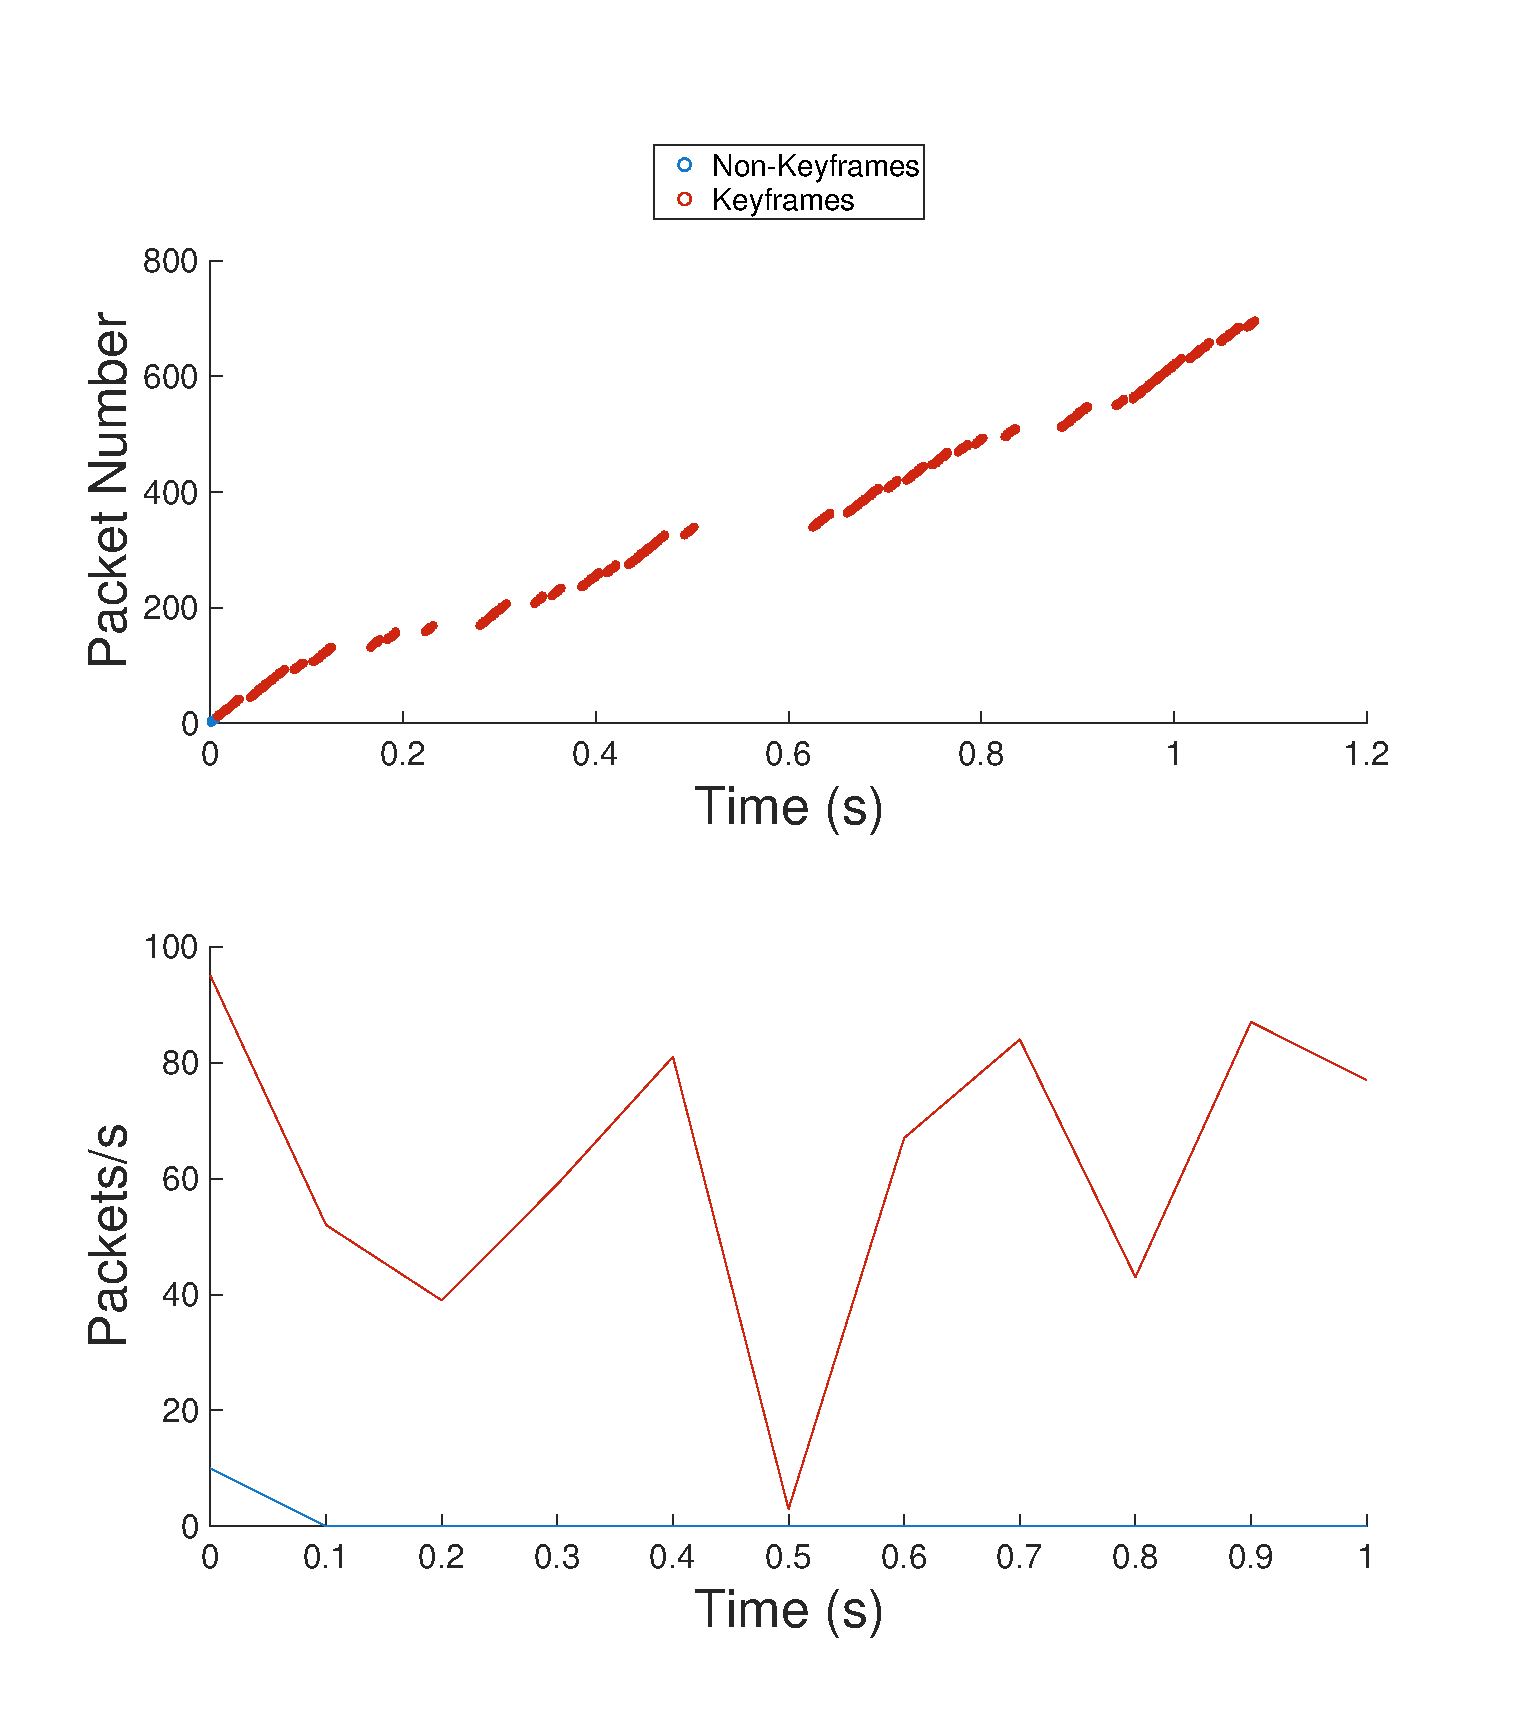
\includegraphics[scale = 0.55]{nocross_slow_16_1}
\caption{No cross-traffic; Slow Channel (Path A : 16 Mbps, Path B : 1 Mbps), measured at the end of Path B}
\end{figure}

\begin{figure}[!h]
\centering
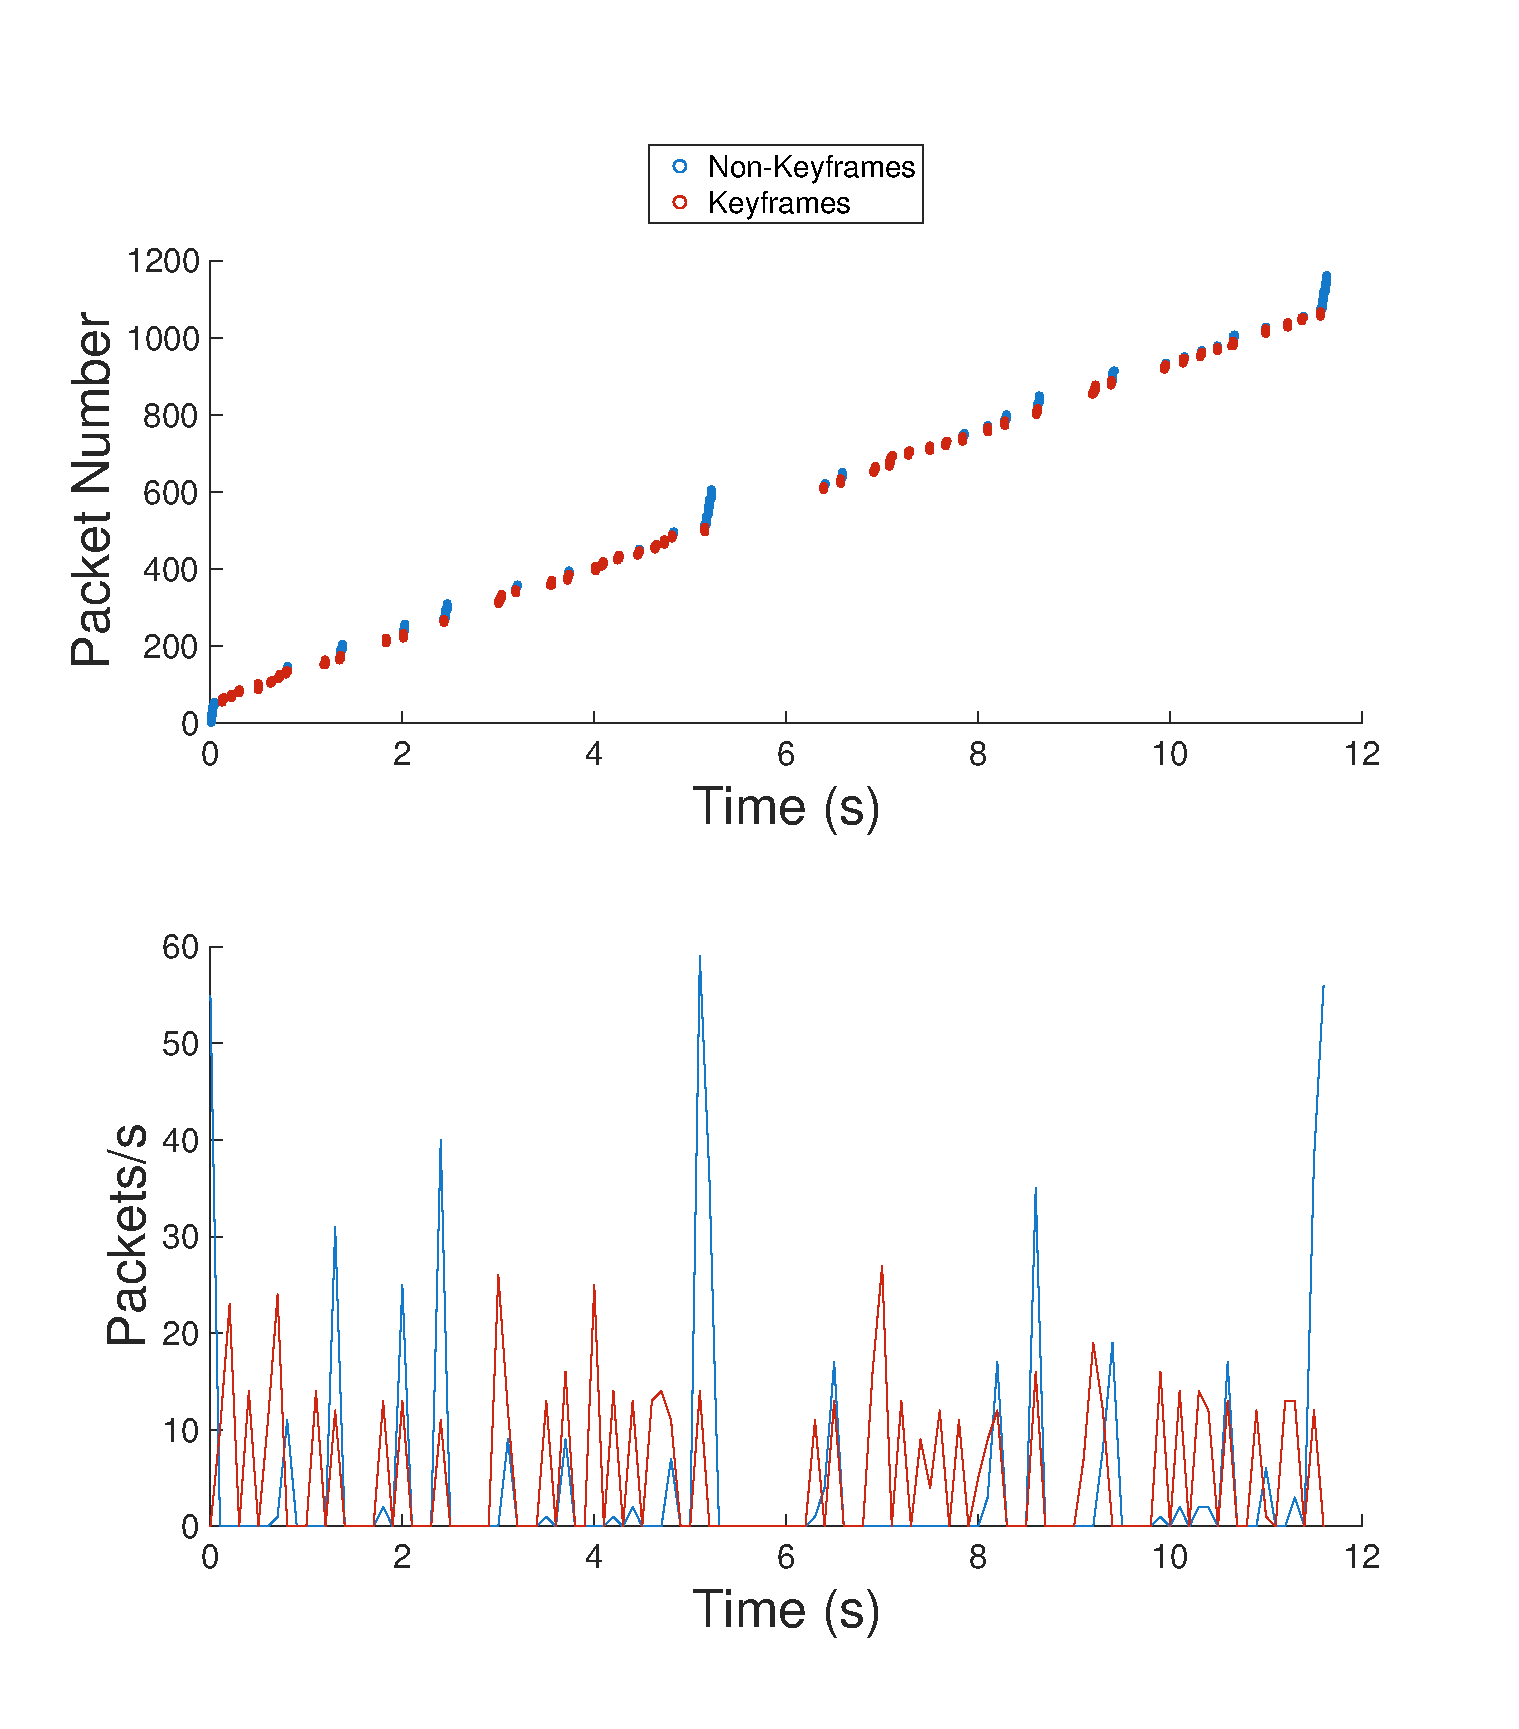
\includegraphics[scale = 0.55]{nocross_med_16_1}
\caption{No cross-traffic; Medium Channel (Path A : 16 Mbps, Path B : 1 Mbps), measured at the end of Path B}
\end{figure}

A preliminary look at the data for this path shows a very important difference with the video traces before entering the flusher. In the case of the slow channel, the keyframe percentage jumps from 46.9\% of all incoming packets to 98.6\%, more than a twofold increase. In the case of the medium channel the increase is even more drastic, going from 4.0\% all the way up to 54.3\%, thus increasing by a factor larger than 12.

Despite this, the amount of \textit{keyframes} remains constant, correctly sending the packet sniffer all packets that it receives. The time elapsed also suffers no perceptible change compared to the case with no buffer flushing, despite the high activity of the flusher.

A particularly interesting observation in both Figure 4.1 and 4.2 is the large gap of packets sent around the middle of the time axis. This corresponds to one of the largest buffer flushes that take place, a fact that one can easily corroborate by looking at the amount of \textit{non-keyframes} that fill that gap in other bandwidth combinations (see Appendix B). In terms of video frames, this would probably signify a relatively long scene showing very similar images from frame to frame.

\clearpage

\subsection{Random cross-traffic}

As previously mentioned, these tests were run by occupying a certain percentage of the channel capacity with random bursts of packets. In this section we discuss the case of 50\% channel occupation to illustrate overall observations. The other results are included in the repository \textit{test\_results} and exhibit very similar results.

\begin{table}[htbp]
\break
\setlength{\arrayrulewidth}{1mm}
\setlength{\tabcolsep}{12pt}
\renewcommand{\arraystretch}{1.5}
 {\rowcolors{3}{whitesmoke}{silver}
\begin{tabular}{ |p{1.375cm}|p{1.375cm}|p{1.25cm}|p{1.5cm}|p{1.5cm}|p{1.75cm}|p{1.5cm}| }
\hline
\textcolor{orange}{BW A} (Mbps)&\textcolor{violet}{BW B} (Mbps)& Total packages & \textit{Keyframe} packages & Keyframe \% & \textit{Non-Keyframe} Packages & Time elapsed (sec) \\
\hline
\multicolumn{7}{|c|}{Slow Channel} \\
\hline
1&4&1465&687&46.9\%&778&35.6\\
16&1&710&687&96.8\%&23&2.3\\
16&16&1465&687&46.9\%&778&2.2\\
\hline
\rowcolor{white}\multicolumn{7}{|c|}{Medium Channel} \\
\hline
1&4&15677&632&4.0\%&15045&371.8\\
16&1&2195&632&28.8\%&1563&23.8\\
16&16&15677&633&4.0\%&15046&23.7\\
\hline
\end{tabular}
}
\caption{Random cross-traffic, 50\% channel occupation}
\end{table}

As can be ascertained from Table 4.3, the operation of the flusher is extremely similar to the case without cross-traffic. The similarity between the first and third bandwidth combinations is roughly maintained, including the ratio between their two elapsed times.

The first of the two largest differences is the differences in time elapsed, both in the slow and the medium channel. The transmitted video traces take around twice as long to be ready to be transmitted, compared to the first case observed. This is, naturally, due to the channel occupation rate, evident in the neat correspondence between a twofold increase in time and a halving of the available channel. 


\begin{figure}[!h]
\centering
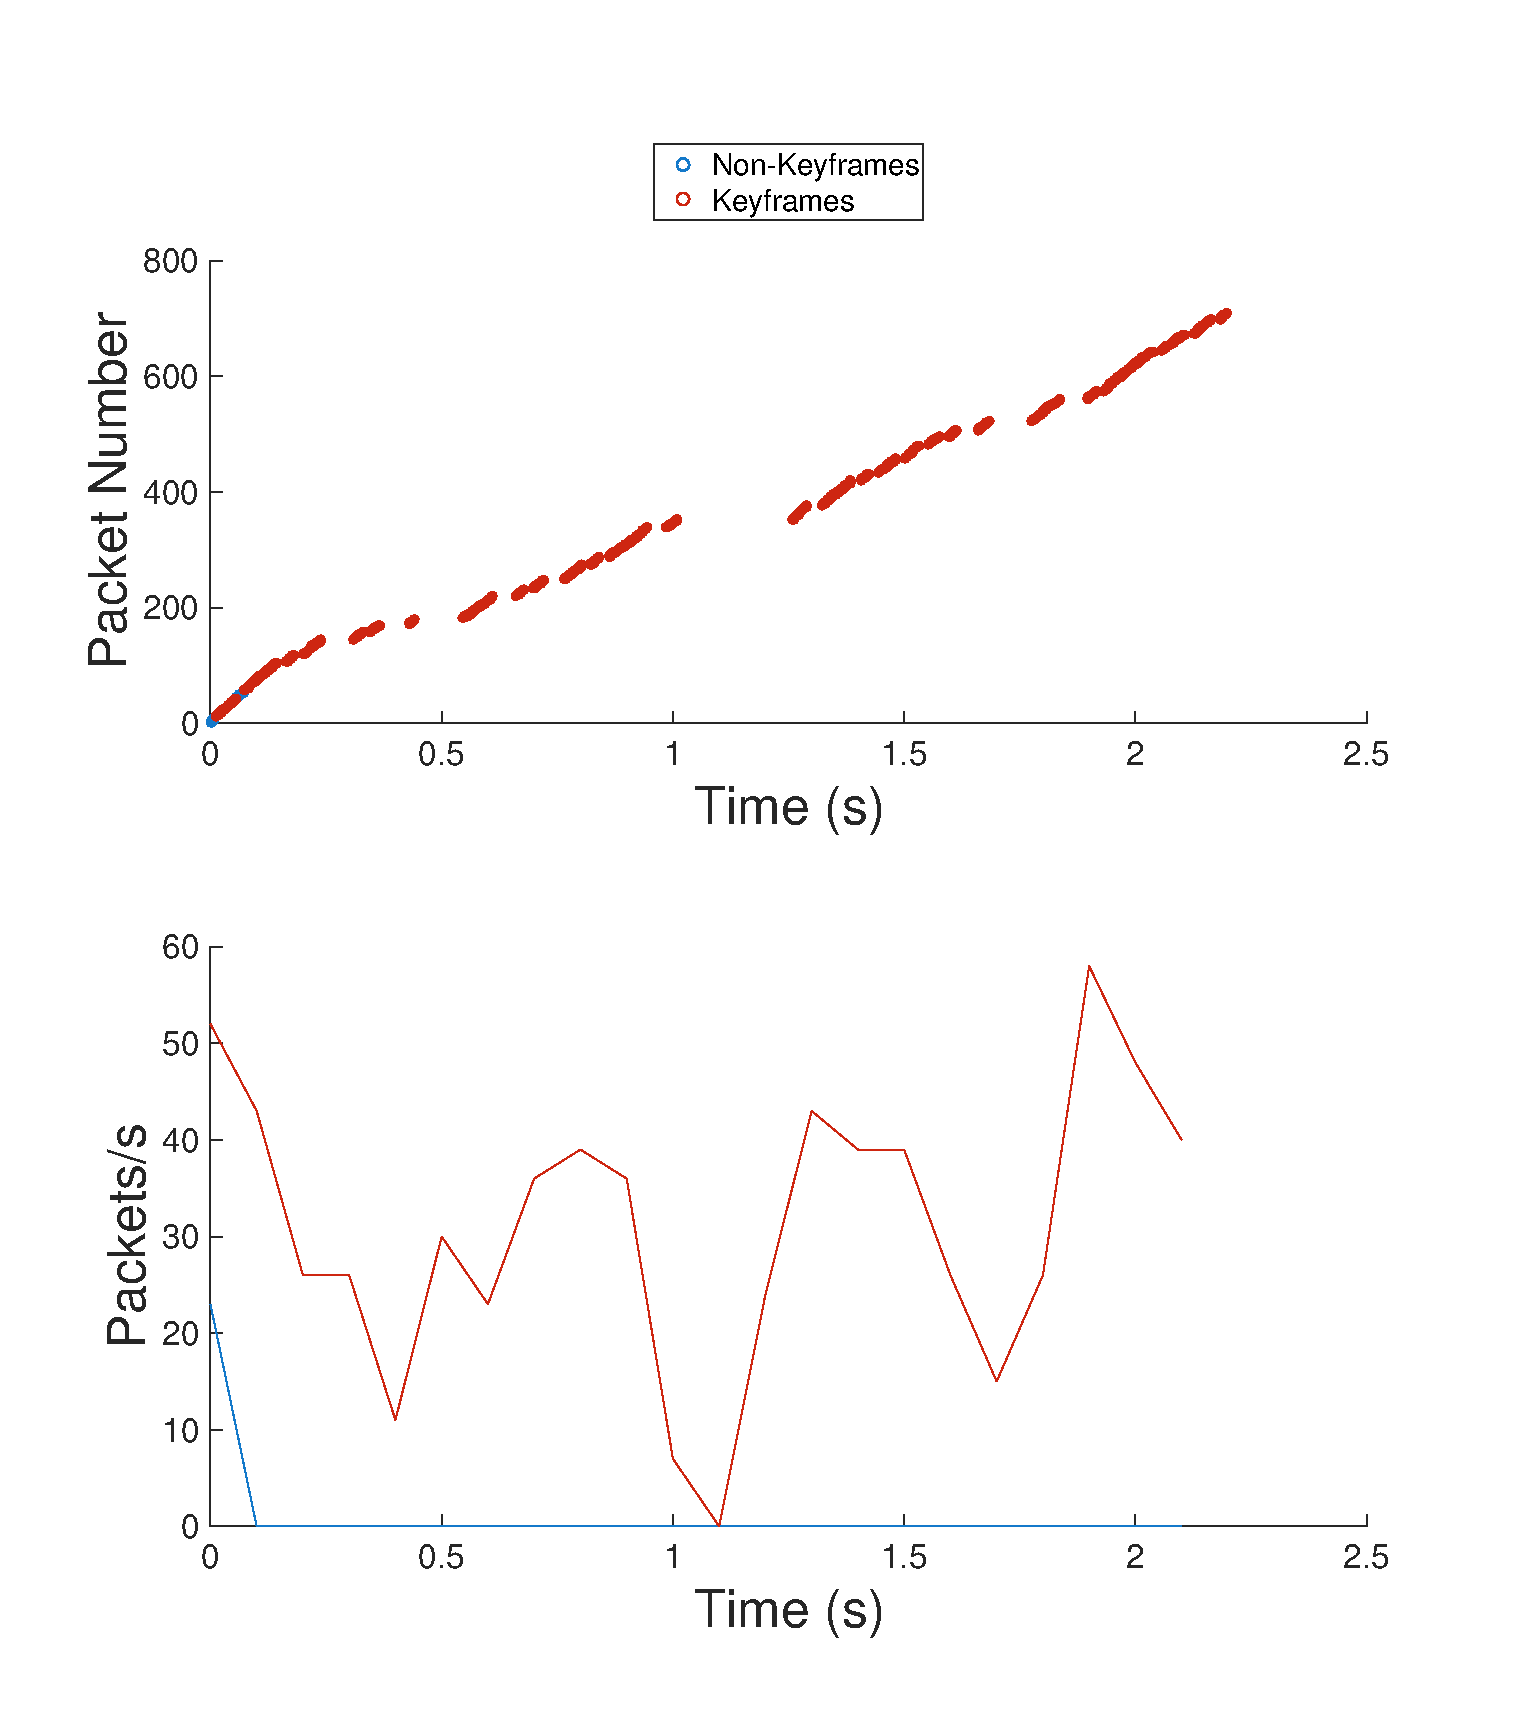
\includegraphics[scale = 0.55]{rand_slow_16_1_50}
\caption{Random cross-traffic; Slow Channel (Path A : 16 Mbps, Path B : 1 Mbps), 50\% channel occupation rate, measured at the end of Path B}
\end{figure}

\begin{figure}[!h]
\centering
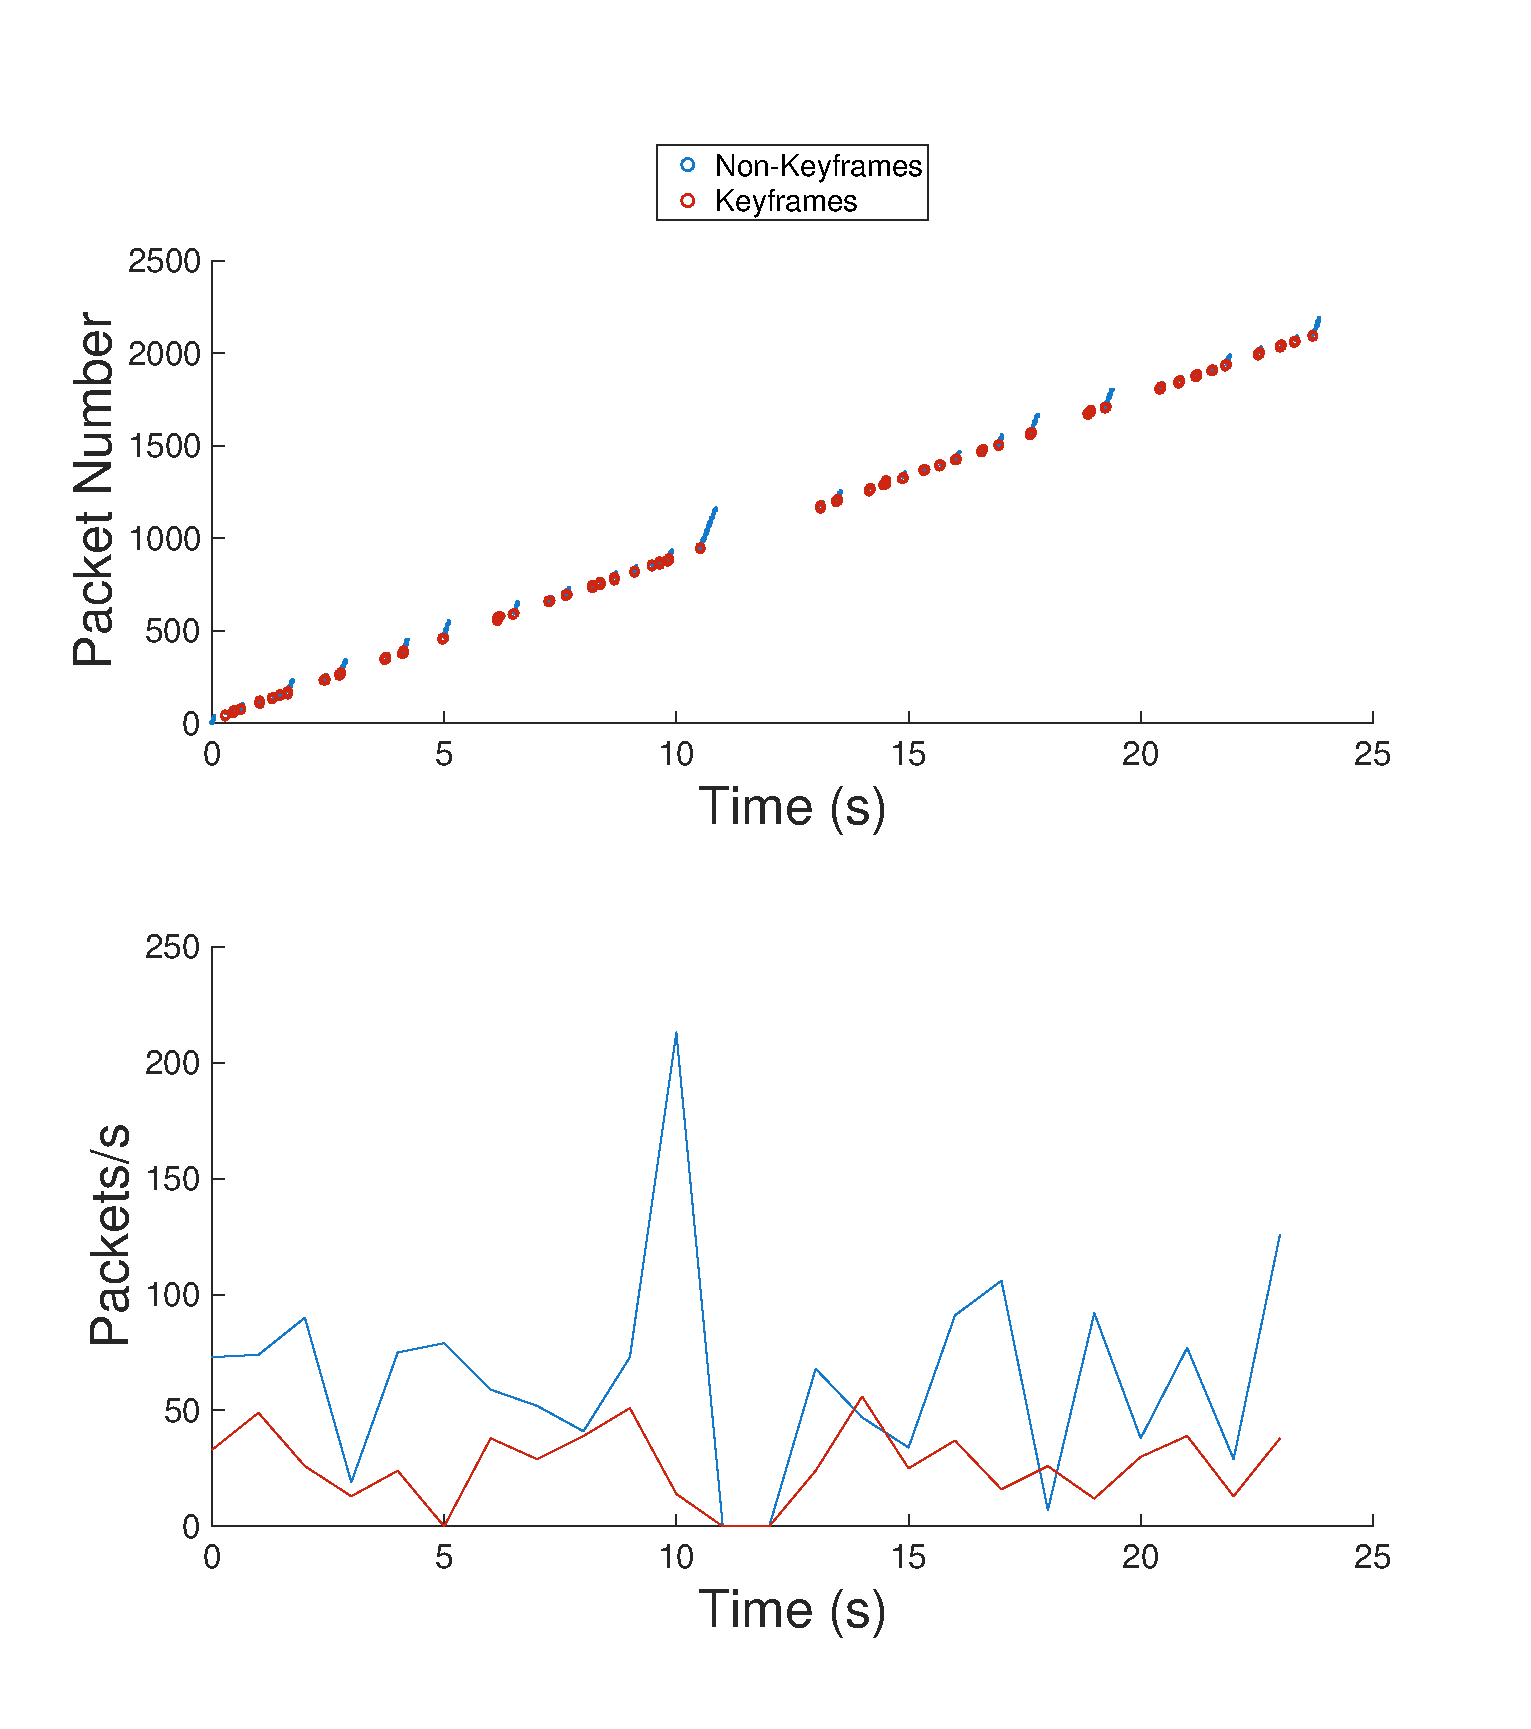
\includegraphics[scale = 0.55]{rand_med_16_1_50}
\caption{Random cross-traffic; Medium Channel (Path A : 16 Mbps, Path B : 1 Mbps), 50\% channel occupation rate, measured at the end of Path B}
\end{figure}

The second difference lies in the case with active buffer flushing. Note the fact that in no occasion is the absolute amount of \textit{keyframe} packets lower than expected: all of them continued to be ready to be transmitted as expected, with no drops. It is the relative percentage of \textit{keyframe} packets that sinks compared to the first set of measurements.

In the slow channel, the relatively low amount of overall packages masks this phenomenon, with a change of only 1.8\% between both sets. In the medium channel, however, the difference is 25.5\%. The reason lies in the effectively lower bandwidth with which the buffer flusher receives packages from the channel. With a lower incoming rate, the flusher triggers less frequently, thus letting more \textit{non-keyframe} packages through. Thus, despite small disruption, the application still exhibits the expected function.

\clearpage

\subsection{Sample pattern of cross-traffic}

Finally, the third set of measurements was performed with background channel traffic corresponding to a packet capture synthesized especially for this purpose and designed to resemble a normal usage of the channel by some other application. The file containing the capture was uploaded to the network emulator, where it was replayed along with the packet transfer. 

A graphic representation of the sample can be seen in Figure 4.5.

\begin{figure}[!ht]
\caption{Sample cross-traffic}
\centering
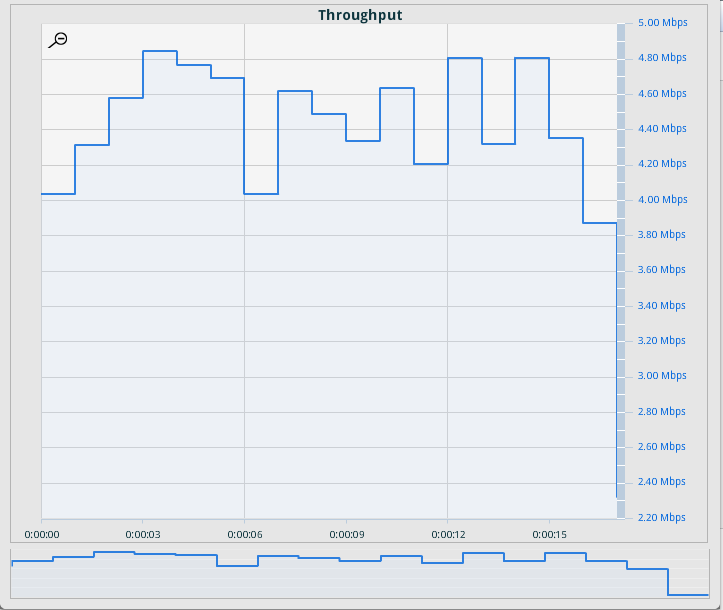
\includegraphics[width = \textwidth]{crosstraffic}
\end{figure}

A glancing look at Table 4.4 reveals very familiar numbers, evidencing the similarity between this measurement set and the first.

\begin{table}[htbp]
\break
\setlength{\arrayrulewidth}{1mm}
\setlength{\tabcolsep}{12pt}
\renewcommand{\arraystretch}{1.5}
 {\rowcolors{3}{whitesmoke}{silver}
\begin{tabular}{ |p{1.375cm}|p{1.375cm}|p{1.25cm}|p{1.5cm}|p{1.5cm}|p{1.75cm}|p{1.5cm}| }
\hline
\textcolor{orange}{BW A} (Mbps)&\textcolor{violet}{BW B} (Mbps)& Total packages & \textit{Keyframe} packages & Keyframe \% & \textit{Non-Keyframe} Packages & Time elapsed (sec) \\
\hline
\multicolumn{7}{|c|}{Slow Channel} \\
\hline
1&4&1465&687&46.9\%&778&17.5\\
16&1&710&687&96.8\%&23&1.2\\
16&16&1465&687&46.9\%&778&1.2\\
\hline
\rowcolor{white}\multicolumn{7}{|c|}{Medium Channel} \\
\hline
1&4&15677&632&4.0\%&15045&191.5\\
16&1&1234&632&51.2\%&602&12.4\\
16&16&15677&632&4.0\%&15046&12.5\\
\hline
\end{tabular}
}
\caption{Sample cross-traffic}
\end{table}

In this set, the phenomena already discussed in the previous two are replicated. The amount of \textit{keyframe} packets remains the same, without any drops. The percentage of \textit{keyframes} compared to the overall packets is much closer to that of the first, unhindered transmission, with a very small dent that can be explained by the rate of channel utilization.

\begin{figure}[!h]
\centering
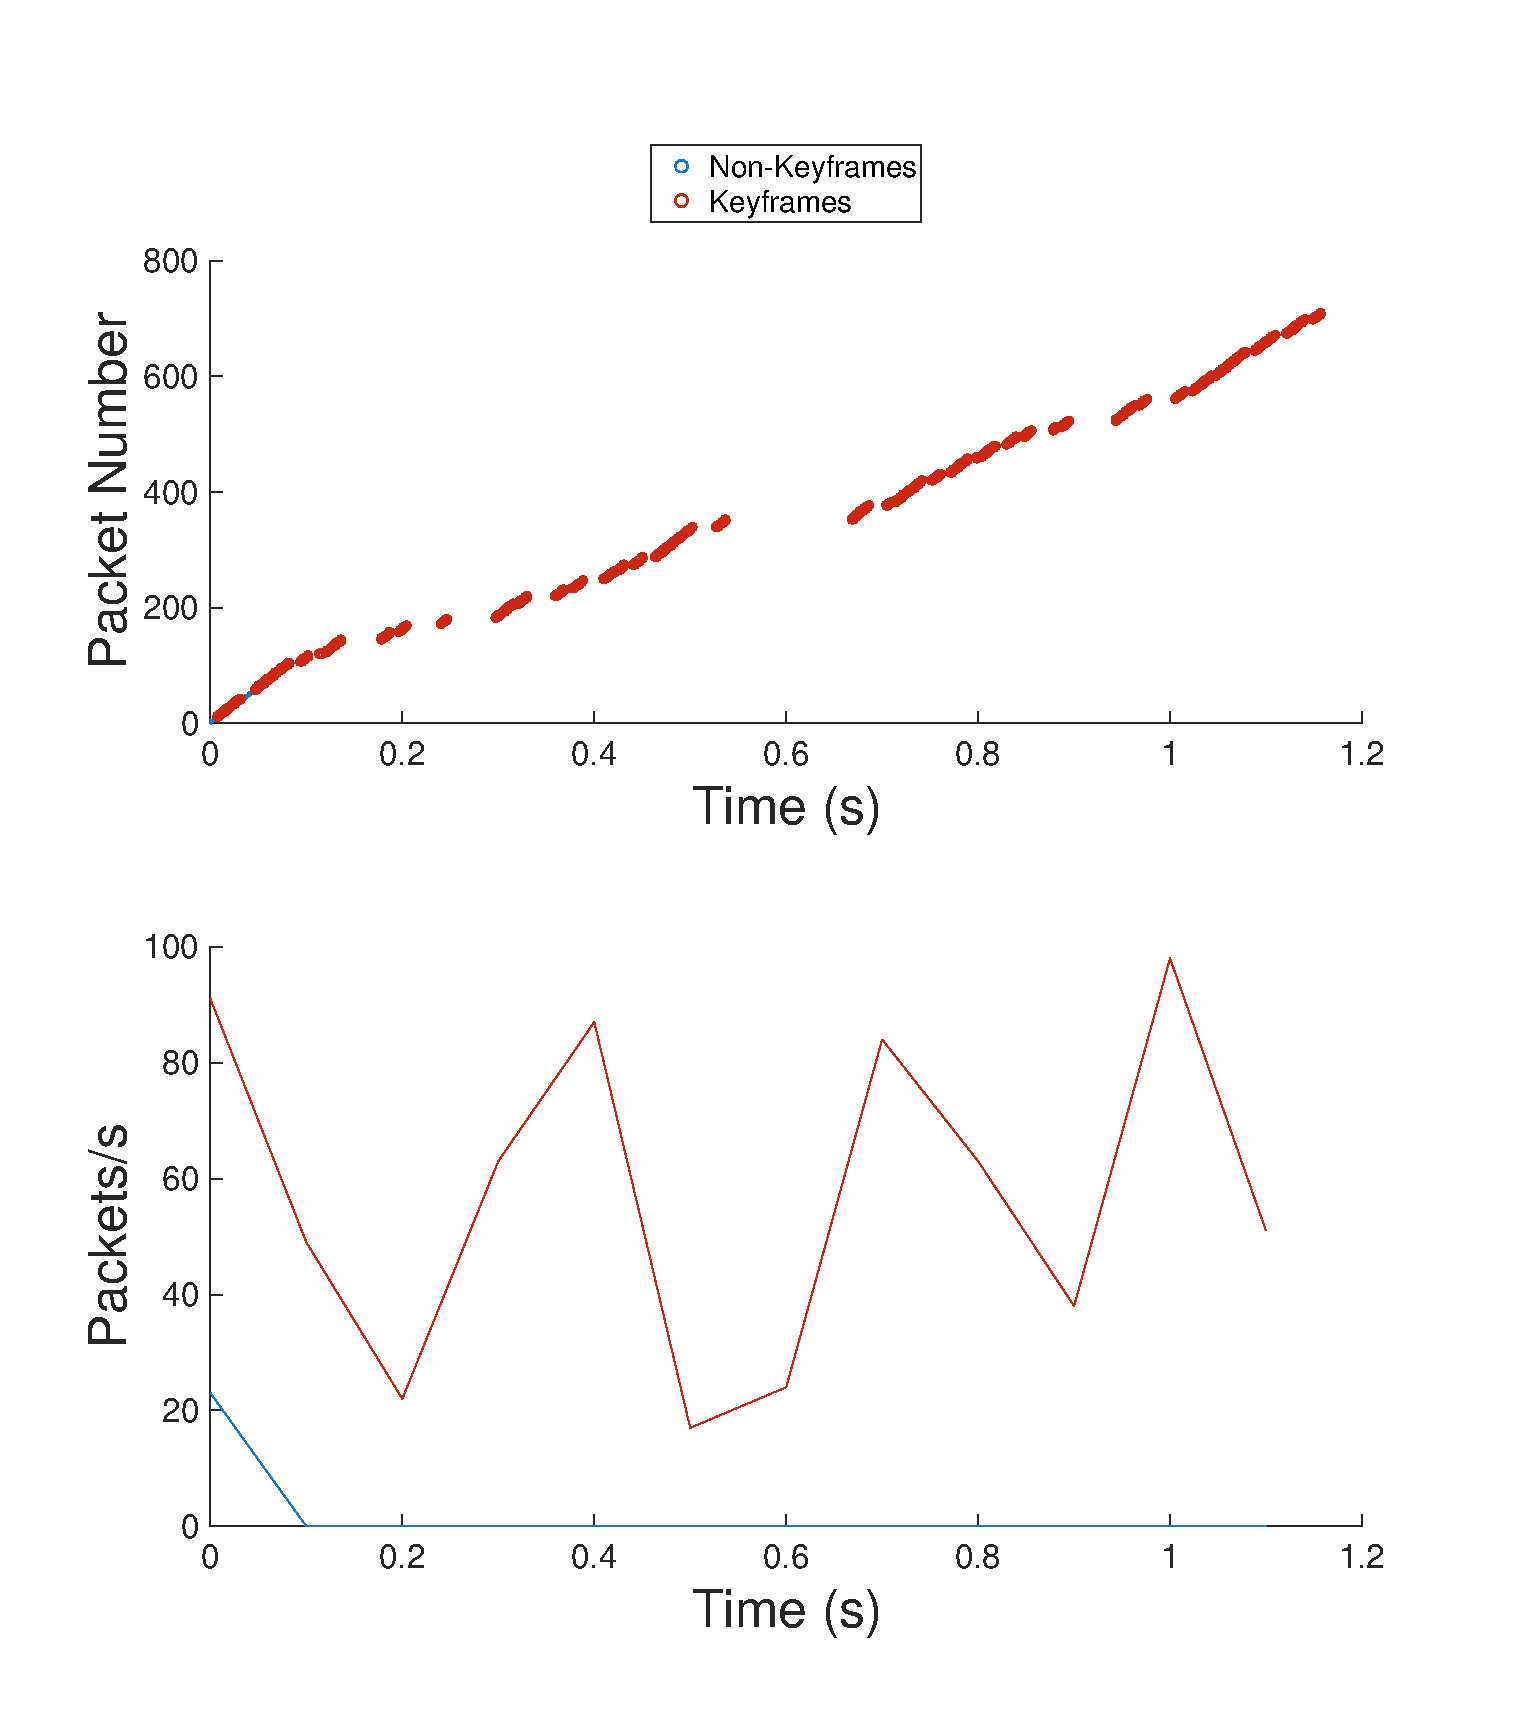
\includegraphics[scale = 0.55]{sample_slow_16_1}
\caption{Sample cross-traffic ; Slow Channel (Path A : 16 Mbps, Path B : 1 Mbps), measured at the end of Path B}
\end{figure}

\begin{figure}[!h]
\centering
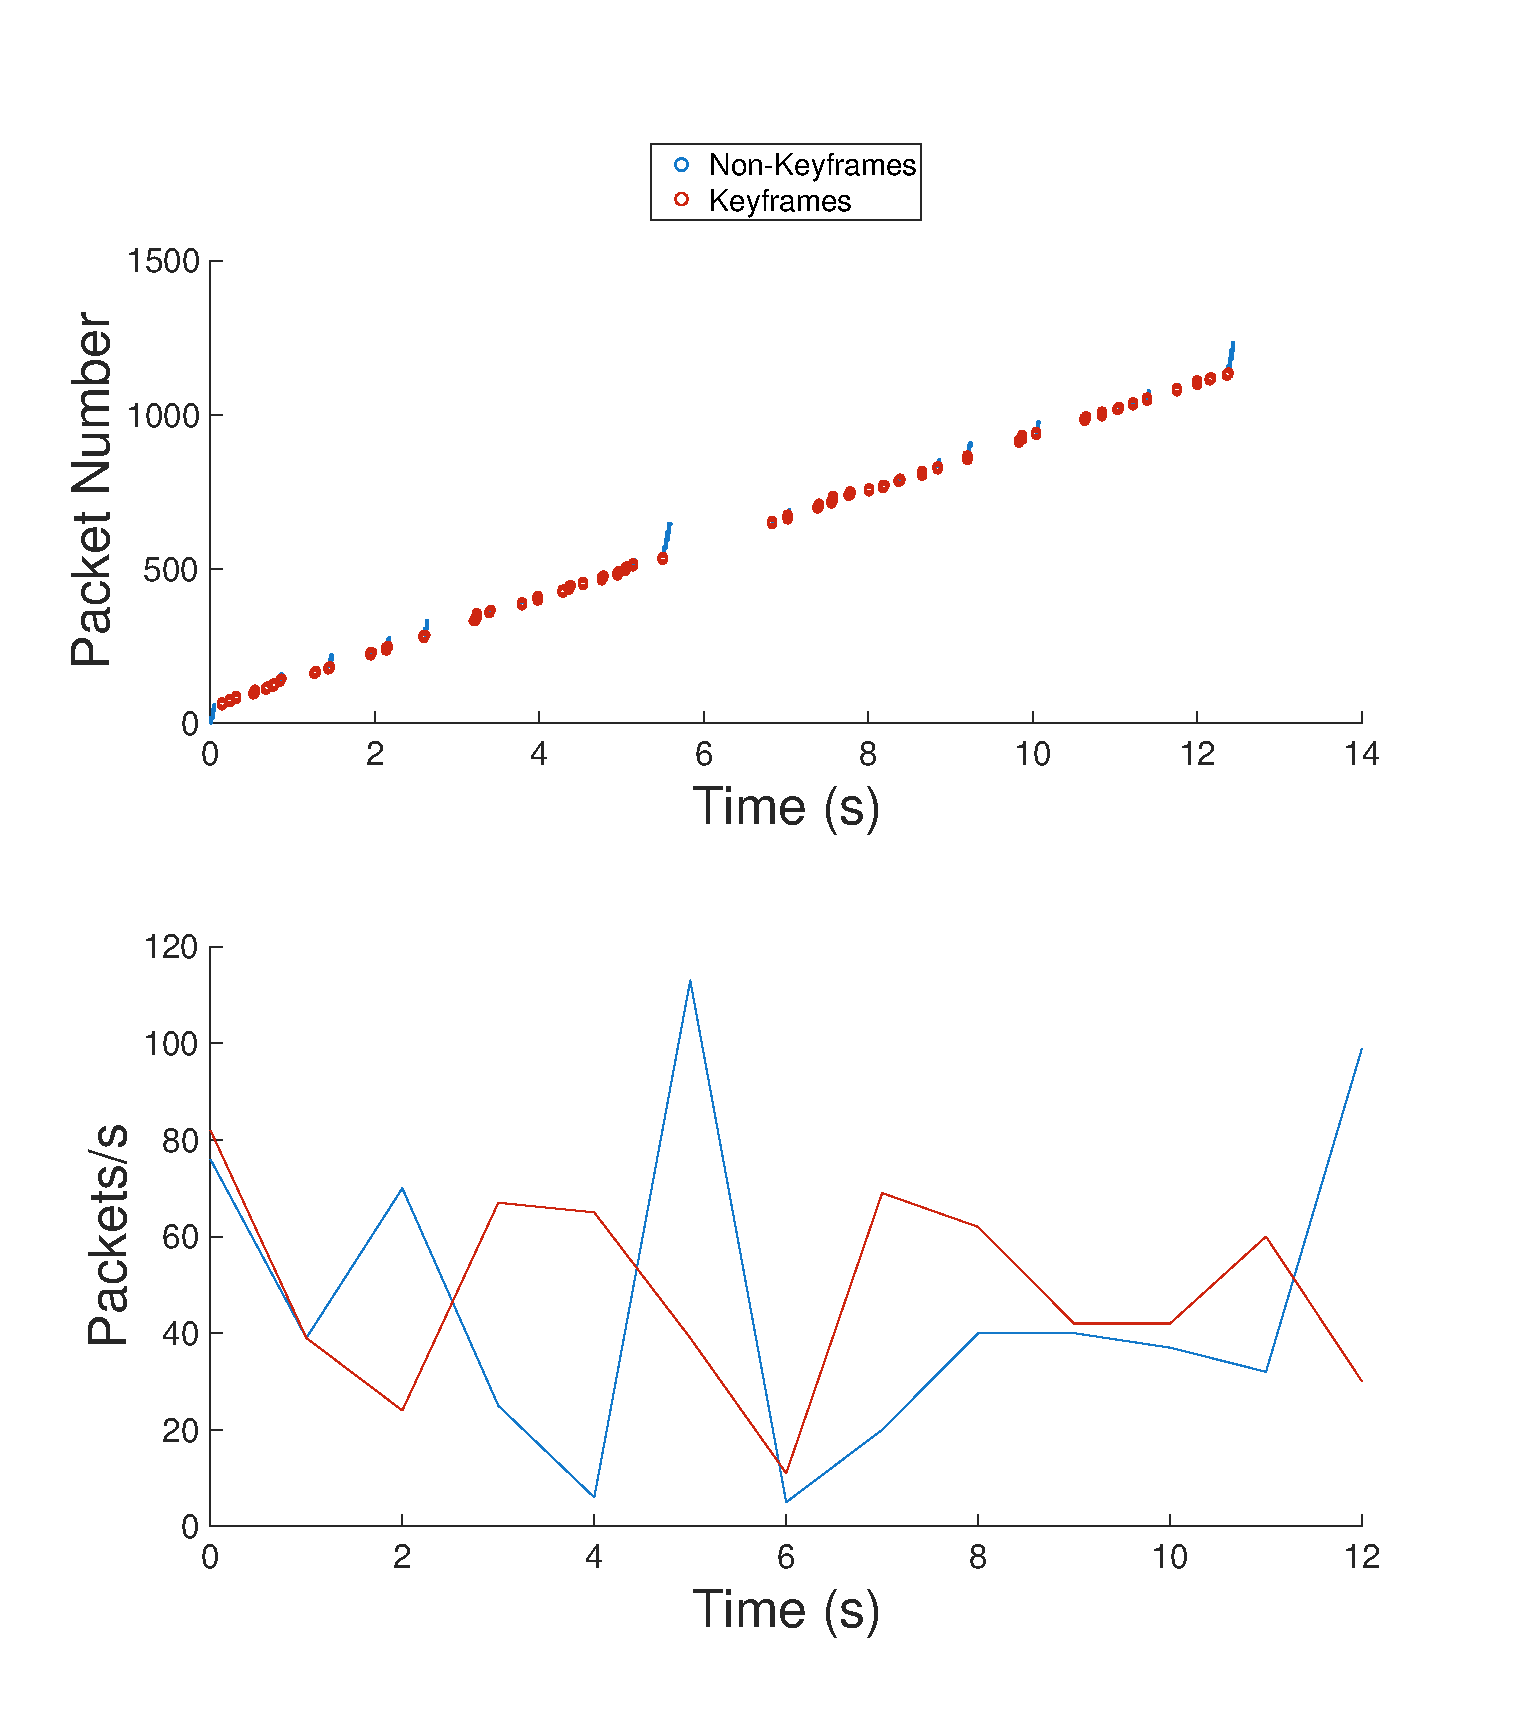
\includegraphics[scale = 0.55]{sample_med_16_1}
\caption{Sample cross-traffic ; Medium Channel (Path A : 16 Mbps, Path B : 1 Mbps), measured at the end of Path B}
\end{figure}

The graphs in Figures 4.6 and 4.7 exhibit a slightly more erratic behavior compared both to the first and second measurement sets, most probably due to the fact that the background traffic exhibits more variation than in the Poisson-distributed random cross-traffic case. Despite this, the overall trends remain constant. 

\clearpage

\chapter{Conclusions}

In the course of our testing, we have observed the performance of a buffer flusher for packets of video frames under different constraints. These have included different combinations of incoming and outgoing data rates as well as various forms of channel occupancy between packet creation and the buffer flusher. 

An effort was also made to leave behind documentation (both for Click and the packet creation scripts) in order to facilitate further work in this topic and alleviate the learning curve associated with the software. These include a small introduction to Click as a whole, with instructions for installation and setup, small tips for monitoring of the packet flow, as well as creation and running of new router configuration files.

The developed buffer flusher has demonstrated the capacity to process large amounts of packets in varying time frames, effectively flushing those with lower priority when the need arises. Additionaly, none of the \textit{keyframes} were dropped in any experiment. 

The effectiveness of the ultimate goal, which is the reduction of the overall transmitted data necessary to transfer all the \textit{keyframes} from one service to the other, can be easily calculated. Table 4.5 illustrates this using the results from the second measurement set.

\begin{table}[htbp]
\break
\setlength{\arrayrulewidth}{1mm}
\setlength{\tabcolsep}{12pt}
\renewcommand{\arraystretch}{1.5}
 {\rowcolors{2}{whitesmoke}{silver}
\begin{tabular}{ |p{3cm}|p{3cm}|p{3cm}|p{3cm}| }
\hline
Channel Type&Total packets&\textit{Keyframe} percentage & File size\\
\hline
\rowcolor{white}\multicolumn{4}{|c|}{Video traces before flushing} \\
\hline
Slow Channel&1465&46.9\%&2.20 MB\\
Medium Channel&15677&4.0\%&23.52 MB\\
\hline
\rowcolor{white}\multicolumn{4}{|c|}{No cross-traffic} \\
\hline
Slow Channel&697&98.6\%&1.05 MB\\
Medium Channel&1163&54.3\%&1.74 MB\\
\hline
\rowcolor{white}\multicolumn{4}{|c|}{Random cross-traffic} \\
\hline
Slow Channel&710&96.8\%&1.07 MB\\
Medium Channel&2195&28.8\%&3.30 MB\\
\hline
\rowcolor{white}\multicolumn{4}{|c|}{Sample cross-traffic} \\
\hline
Slow Channel&710&96.8\%&1.07 MB\\
Medium Channel&1234&51.2\%&1.85 MB\\
\hline
\end{tabular}
}
\caption{File size to be sent after buffer flusher}
\end{table}

As is especially visible in files with a higher percentage of \textit{non-keyframes}, the difference between unadulterated and flushed files is significant, reaching up to a 92.6\% reduction in total file size to be transferred in the case with no cross-traffic.

All of the observations described in this report also reflect the measurements not discussed here due to concerns for repetitiveness or readability. For the packet capture files of these other measurements please refer to the \textit{test\_results} repository.

Thus we have fulfilled all the initial goals of the project except for the integration with the Linux kernel, which was deemed out of the time scope of this Engineer practice.